\documentclass[10pt,xcolor=pst,aspectratio=169]{beamer}

\usepackage{etex}

%\usetheme{Boadilla}
%\usecolortheme{wolverine}
\usecolortheme{dolphin}
%\setbeamercovered{transparent}
%\setbeamercolor{block body}{bg=yellow}

\addtobeamertemplate{navigation symbols}{}{%
\usebeamerfont{footline}%
\usebeamercolor[fg]{footline}%
\hspace{1em}%
\insertframenumber/\inserttotalframenumber
}

\usepackage[utf8]{inputenc}
\usepackage[english,russian]{babel}
\usepackage[OT1]{fontenc}
\usepackage{amsmath, bm}
\usepackage{amsfonts}
\usepackage{amssymb}
\usepackage{graphicx}
\usepackage{wrapfig}
\usepackage[3D]{movie15}
\usepackage{ragged2e}
\usepackage{listings}
\usepackage{color}
\usepackage{pst-all}

\usepackage{tikz}
\usetikzlibrary{
    mindmap,
    arrows, % стрелки
    shapes.misc, % фигуры
    chains, % цепочки
    positioning, % позиционирование элементов
    scopes, % создание дополнительных веток
    shadows % тени
    }

\graphicspath{{pic/}}

\author{\textbf{Губкин А.С.}}

\title[Численные методы в физике]{Численные методы в физике}

\logo{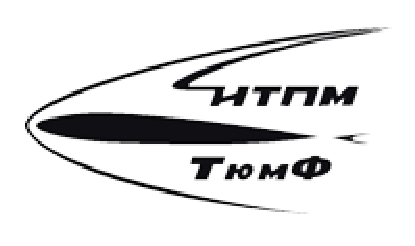
\includegraphics[width=0.1\linewidth]{LOGO_2.EPS}}

\institute[ТюмФ ИТПМ СО РАН]{Тюменский филиал Института теоретической и прикладной механики\\ им. С. А. Христиановича СО РАН, г. Тюмень}

\date{6 октября 2015 г.}

\begin{document}

\lstset{ %
    language=[ANSI]C++,                 % выбор языка для подсветки (здесь это С++)
    keywordstyle=\color{blue},
    commentstyle=\color{gray},
    basicstyle=\scriptsize,
%basicstyle=\small\sffamily, % размер и начертание шрифта для подсветки кода
    numbers=left,               % где поставить нумерацию строк (слева\справа)
    numberstyle=\tiny,           % размер шрифта для номеров строк
%stepnumber=1,                   % размер шага между двумя номерами строк
    numbersep=4pt,                % как далеко отстоят номера строк от подсвечиваемого кода
%backgroundcolor=\color{white}, % цвет фона подсветки - используем \usepackage{color}
    showspaces=false,            % показывать или нет пробелы специальными отступами
    showstringspaces=false,      % показывать или нет пробелы в строках
    showtabs=false,             % показывать или нет табуляцию в строках
    frame=single,              % рисовать рамку вокруг кода
%tabsize=2,                 % размер табуляции по умолчанию равен 2 пробелам
    captionpos=t,              % позиция заголовка вверху [t] или внизу [b] 
    breaklines=true,           % автоматически переносить строки (да\нет)
    breakatwhitespace=true, % переносить строки только если есть пробел
    escapeinside={\%*}{*)}   % если нужно добавить комментарии в коде
}

%SLIDE #
\begin{frame}

    \transdissolve[duration=0.1]
    \titlepage

\end{frame}

%SLIDE #
\begin{frame}{Литература}

    \transdissolve[duration=0.1]

    \begin{itemize}
        \item Андерсон Д., Таннехилл Дж., Плетчер Р. Вычислительная гидродинамика и теплообмен. Том 1,2 (1990).

        \item Зализняк В.Е. Численные методы. Основы научных вычислений. - М.: Издательство Юрайт, 2012. - 356 с.

        \item Формалев В.Ф., Ревезников Д.Л. Численные методы. - М.: ФИЗМАТЛИТ, - 2004. - 400 с.

        \item Рождественский Б.Л., Яненко Н.Н. Системы квазилинейных уравнений и их приложения к газовой динамике (2-е изд.). - М.: Наука, 1978. - 688 с.
        
        \item Жуков М.Ю. Квазилинейные гиперболические уравнения: Учебно-методическое пособие. - Ростов-на-Дону, 2008. - 52 с.

        \item Куликовский А.Г., Погорелов Н.В., Семенов А.Ю. Математические вопросы численного решения гиперболических систем уравнений. - М.: ФИЗМАТЛИТ, 2012. - 656 с.

        \item Лейбович С., Сибасс А. (ред.) Нелинейные волны. - М.: Мир, 1977.
    \end{itemize}

    и др.

\end{frame}

%SLIDE #
\begin{frame}{Введение}

    \transdissolve[duration=0.1]
    \justifying
    \large

    Многие физические проблемы сводятся к решению \textbf{уравнений в частных производных}, поэтому необходимо знать физические особенности решений этих уравнений. Для решения конкретных задач необходимо уметь определять тип дифференциального уравнения в частных производных и знать его основные математические особенности.

\end{frame}

%SLIDE #
\begin{frame}{Уравнение в частных производных}

    \transdissolve[duration=0.1]
    \justifying
    \large

    Уравнением в частных производных относительно функции $u \left( \mathbf{x} \right)$ называется уравнение вида:

    \[
        f \left( \mathbf{x}, u, \bm{\nabla} u, \bm{\nabla} \bm{\nabla} u, \ldots \right) = 0.
    \]

\end{frame}

%SLIDE #
\begin{frame}{Физическая классификация уравнений}

    \transdissolve[duration=0.1]
    \justifying
    \large

%   \begin{center}
%       \begin{tikzpicture}[edge from parent fork down]
%           \tikzstyle{every node}=[fill=yellow!150, rounded corners]
%           \tikzstyle{edge from parent}=[blue, -*, thick,draw]
%           \tikzstyle{level 1}=[level distance=2cm, sibling distance=4cm]
%           
%           \node {Задачи для УЧП}
%               child {node {Маршевые}}
%               child {node {Стационарные}};
%       \end{tikzpicture}
%   \end{center}
    
    \begin{center}
        \tikzstyle{root concept}+=[concept color=blue!80,minimum size=3cm]
        \tikz[mindmap]
            \node [concept] {Задачи для УЧП}
                child[concept color=yellow, grow=135, minimum size=2cm]
                {
                    node[concept](root1) at (1,0) {Маршевые} node[annotation,left] at (0,0)
                    {
                        \begin{itemize}
                            \item нестационарные течения невязкой/вязкой жидкости;
                            \item стационарные сверхзвуковые течения невязкого/вязкого газа;
                            \item пограничный слой;
                            \item нестационарное распространение тепла, и т.д.
                        \end{itemize}
                    }
                }
                child[concept color=green, grow=45, minimum size=2cm] 
                {
                    node[concept](root2) at (-1,0) {Стацио\-нарные} node[annotation,right] at (0,0)
                    {
                        \begin{itemize}
                            \item стационарные течения невязкой/вязкой жидкости;
                            \item стационарные сверхзвуковые течения невязкого/вязкого газа;
                            \item стационарные задачи теплопроводности, и т.д.
                        \end{itemize}
                    }
                };
    \end{center}

\end{frame}

%SLIDE #
\begin{frame}{Маршевые задачи}

    \transdissolve[duration=0.1]
    \justifying
    \large

    \textbf{Маршевой} или \textbf{эволюционной} (или задачей распространения) называется задача, в которой требуется найти решение уравнения в частных производных в \textbf{незамкнутой области} при заданных граничных и начальных условиях.\\

    Решение таких задач должно быть найдено последовательным движением в маршевом направлении. Такие задачи описываются уравнениями в частных производных \textbf{гиперболического} или \textbf{параболического} типа.

\end{frame}

%SLIDE #
\begin{frame}{Стационарные}

    \transdissolve[duration=0.1]
    \justifying
    \large

    Задача называется \textbf{стационарной}, если решение уравнения в частных производных внутри некоторой области определяется лишь условиями на границе этой области\\

    Физически стационарная задача описывает установившийся процесс, а математически сводится к решению задачи с граничными условиями (краевой задачи) для уравнения в частных производных.\\

    Иногда стационарные задачи называют \textbf{детерминированными}, так как решение в любой внутренней точке области определяется условиями, заданными на ее границе.

\end{frame}

%SLIDE #
\begin{frame}{Уравнения характерные для маршевых задач}

    \transdissolve[duration=0.1]
    \justifying
    \large

    Волновое уравнение:

    \[
        a(\mathbf{x}) \frac{\partial^{2} u}{\partial t^{2}} = \bm{\nabla} \cdot \left( b(\mathbf{x}) \bm{\nabla} u \right) - c(\mathbf{x}) u + f(\mathbf{x}, t).
    \]

    Уравнение теплопроводности (диффузии):

    \[
        a(\mathbf{x}) \frac{\partial u}{\partial t} = \bm{\nabla} \cdot \left( b(\mathbf{x}) \bm{\nabla} u \right) - c(\mathbf{x}) u + f(\mathbf{x}, t).
    \]

\end{frame}

%SLIDE #
\begin{frame}{Уравнения характерные для маршевых задач}

    \transdissolve[duration=0.1]
    \justifying
    \large

    Уравнения Максвелла:

    \[
        \begin{split}
            &\bm{\nabla} \cdot \mathbf{D} = \rho (\mathbf{x}), \:
            \bm{\nabla} \cdot \mathbf{B} = 0 \\ 
            &\bm{\nabla} \times \mathbf{E} = - \frac{\partial \mathbf{B}}{\partial t}, \:
            \bm{\nabla} \times \mathbf{H} = \mathbf{j} + \frac{\partial \mathbf{D}}{\partial t}.
        \end{split}
    \]

\end{frame}

%SLIDE #
\begin{frame}{Уравнения характерные для маршевых задач}

    \transdissolve[duration=0.1]
    \justifying
    \large

    Уравнения газо-гидродинамики (уравнения Эйлера):

    \[
        \begin{split}
            &\frac{\partial \rho}{\partial t}
                + \bm{\nabla} \cdot \rho \mathbf{u}
                = 0, \\
            &\frac{\partial \rho \mathbf{u}}{\partial t}
                + \bm{\nabla} \cdot \left( \rho \mathbf{u} \otimes \mathbf{u} + p \mathbf{I} \right)
                =
                \mathbf{F}, \\
            &\frac{\partial \rho E}{\partial t}
                + \bm{\nabla} \cdot \left( \mathbf{u} \left( \rho E + p \right) \right)
                =
                \mathbf{F} \cdot \mathbf{u}.
            \end{split}
    \]

\end{frame}

%SLIDE #
\begin{frame}{Уравнения характерные для маршевых задач}

    \transdissolve[duration=0.1]
    \justifying
    \large

    Уравнения Навье-Стокса:
    \[
        \begin{split}
            &\frac{\partial \rho}{\partial t}
                + \bm{\nabla} \cdot \rho \mathbf{u}
                = 0, \\
            &\frac{\partial \rho \mathbf{u}}{\partial t}
                + \bm{\nabla} \cdot \rho \mathbf{u} \otimes \mathbf{u}
                =
                - \bm{\nabla} p
                + \bm{\nabla} \cdot \bm{\tau}
                + \mathbf{F}, \\
            &\frac{\partial \rho E}{\partial t}
                + \bm{\nabla} \cdot \rho E \mathbf{u}
                =
                \bm{\nabla} \cdot \left( \bm{\sigma} \cdot \mathbf{u} - \mathbf{q} \right)
                + \mathbf{F} \cdot \mathbf{u}.
            \end{split}
    \]

\end{frame}

%SLIDE #
\begin{frame}{Уравнения характерные для стационарных задач}

    \transdissolve[duration=0.1]
    \justifying
    \large

    Волновое уравнение и уравнение диффузии:
   
    \[
        \bm{\nabla} \cdot \left( b(\mathbf{x}) \bm{\nabla} u \right) - c(\mathbf{x}) u + f(\mathbf{x}, t) = 0.
    \]

    Уравнение Гельмгольца:

    \[
        \triangle u_{0} + \frac{\omega^{2}}{c^2} u_{0} = - \frac{f_{0}(\mathbf{x})}{c^{2}}.
    \]

    Уравнения электростатики и магнитостатики:

    \[
        \begin{split}
            &\bm{\nabla} \cdot \mathbf{D} = \rho (\mathbf{x}), \:
            \bm{\nabla} \times \mathbf{E} = 0, \\
            &\bm{\nabla} \cdot \mathbf{B} = 0, \:
            \bm{\nabla} \times \mathbf{H} = \mathbf{j}.
        \end{split}
    \]

\end{frame}

%SLIDE #
\begin{frame}{Постановка основных задач для уравнений математической физики}

    \transdissolve[duration=0.1]
    \justifying
    \large

    Различают три основных типа краевых задач для дифференциальных уравнений в частных производных:

    \begin{itemize}
        \item \textbf{задача Коши} для нестационарных уравнений: задаются начальные условия, граничные условия отсутствуют;

        \item \textbf{краевая задача} для стационарных уравнений: задаются граничные условия, начальные условия отсутствуют;

        \item \textbf{смешаная задача} для нестационарных уравнений: задаются и начальные, и граничные условия.
    \end{itemize}

\end{frame}

%SLIDE #
\begin{frame}{Задача Коши}

    \transdissolve[duration=0.1]
    \justifying
    \large

    \begin{itemize}
        \item Для волнового уравнения второго порядка:
            \[
                u(\mathbf{x}, 0) = f_{0}(\mathbf{x}), \: \left. \frac{\partial u(\mathbf{x}, t)}{\partial t} \right|_{t = 0}= f_{1}(\mathbf{x}).
            \]

        \item Для уравнений диффузии и Шредингера:
            \[
                u(\mathbf{x}, 0) = f_{0}(\mathbf{x}).
            \]

        \item Для системы уравнений первого порядка:
            \[
                \mathbf{u}(\mathbf{x}, 0) = \mathbf{f}_{0}(\mathbf{x}).
            \]
    \end{itemize}

\end{frame}

%SLIDE #
\begin{frame}{Краевая задача для стационарных уравнений}

    \transdissolve[duration=0.1]
    \justifying
    \large

    Для уравнения 

    \[
        \bm{\nabla} \cdot \left( b(\mathbf{x}) \bm{\nabla} u \right) - c(\mathbf{x}) u + f(\mathbf{x}, t) = 0,
    \]

    граничное условие будет иметь вид:

    \[
        \left. \left( \alpha u + \beta \frac{\partial u}{\partial \mathbf{n}} \right) \right|_{s} = g_{0}.
    \]

\end{frame}

%SLIDE #
\begin{frame}{Краевая задача для стационарных уравнений}

    \transdissolve[duration=0.1]
    \justifying
    \large

    Часто встречаются следующие типы граничных условий:

    \begin{itemize}
        \item Граничное условие первого рода ($\alpha = 1, \: \beta = 0$):
            \[
                \left. u \right|_{S} = g_{0}.
            \]

        \item Граничное условие второго рода ($\alpha = 0, \: \beta = 1$):
            \[
                \left. \frac{\partial u}{\partial \mathbf{n}} \right|_{S} = g_{0}.
            \]

        \item Граничное условие третьего рода ($\alpha \geq 0, \: \beta = 1$):
            \[
                \left. \left( \alpha u + \frac{\partial u}{\partial \mathbf{n}} \right) \right|_{S} = g_{0}.
            \]
    \end{itemize}

\end{frame}

%SLIDE #
\begin{frame}{Математическая классификация уравнений}

    \transdissolve[duration=0.1]
    \justifying
    \large

    Уравнение в частных производных второго порядка, записанное в общем виде, обычно используют для пояснения математической классификации уравнений в частных производных. Рассмотрим уравнение в частных производных

    \[
        a \frac{\partial^{2} \phi}{\partial x^{2}} + b \frac{\partial^{2} \phi}{\partial x \partial y} + c \frac{\partial^{2} \phi}{\partial y^{2}} + d \frac{\partial \phi}{\partial x} + e \frac{\partial \phi}{\partial y} + f \phi = g \left( x, y \right).
    \]

    Здесь $a, \: b, \: c, \: d, \: e, \: f$ -- функции от $x$, $y$, т. е. рассматривается лишь линейное уравнение.

\end{frame}

%SLIDE #
\begin{frame}{Математическая классификация уравнений}

    \transdissolve[duration=0.1]
    \justifying
    \large

    Определим теперь \textbf{канонические} формы записи уравнений в частных производных различных типов.\\

    Известно, что предыдущее уравнение может быть трех различных типов в зависимости от знака определителя:

    \[
        \triangle = b^{2} - 4 a c.
    \]

    \begin{itemize}
        \item гиперболическим: $\triangle > 0$;
        \item параболическим: $\triangle = 0$;
        \item эллиптическим: $\triangle < 0$.
    \end{itemize}

\end{frame}

%SLIDE #
\begin{frame}{Геометрическая аналогия}

    \transdissolve[duration=0.1]
    \justifying
    \large

    \vspace{-60pt}

    \[
        A x^{2} + B x y + C y^{2} + D x + E y + F = 0.
    \]

    %FIG. #
    \begin{wrapfigure}[10]{r}[-40pt]{8cm}
        \vspace{-20pt}
        \center{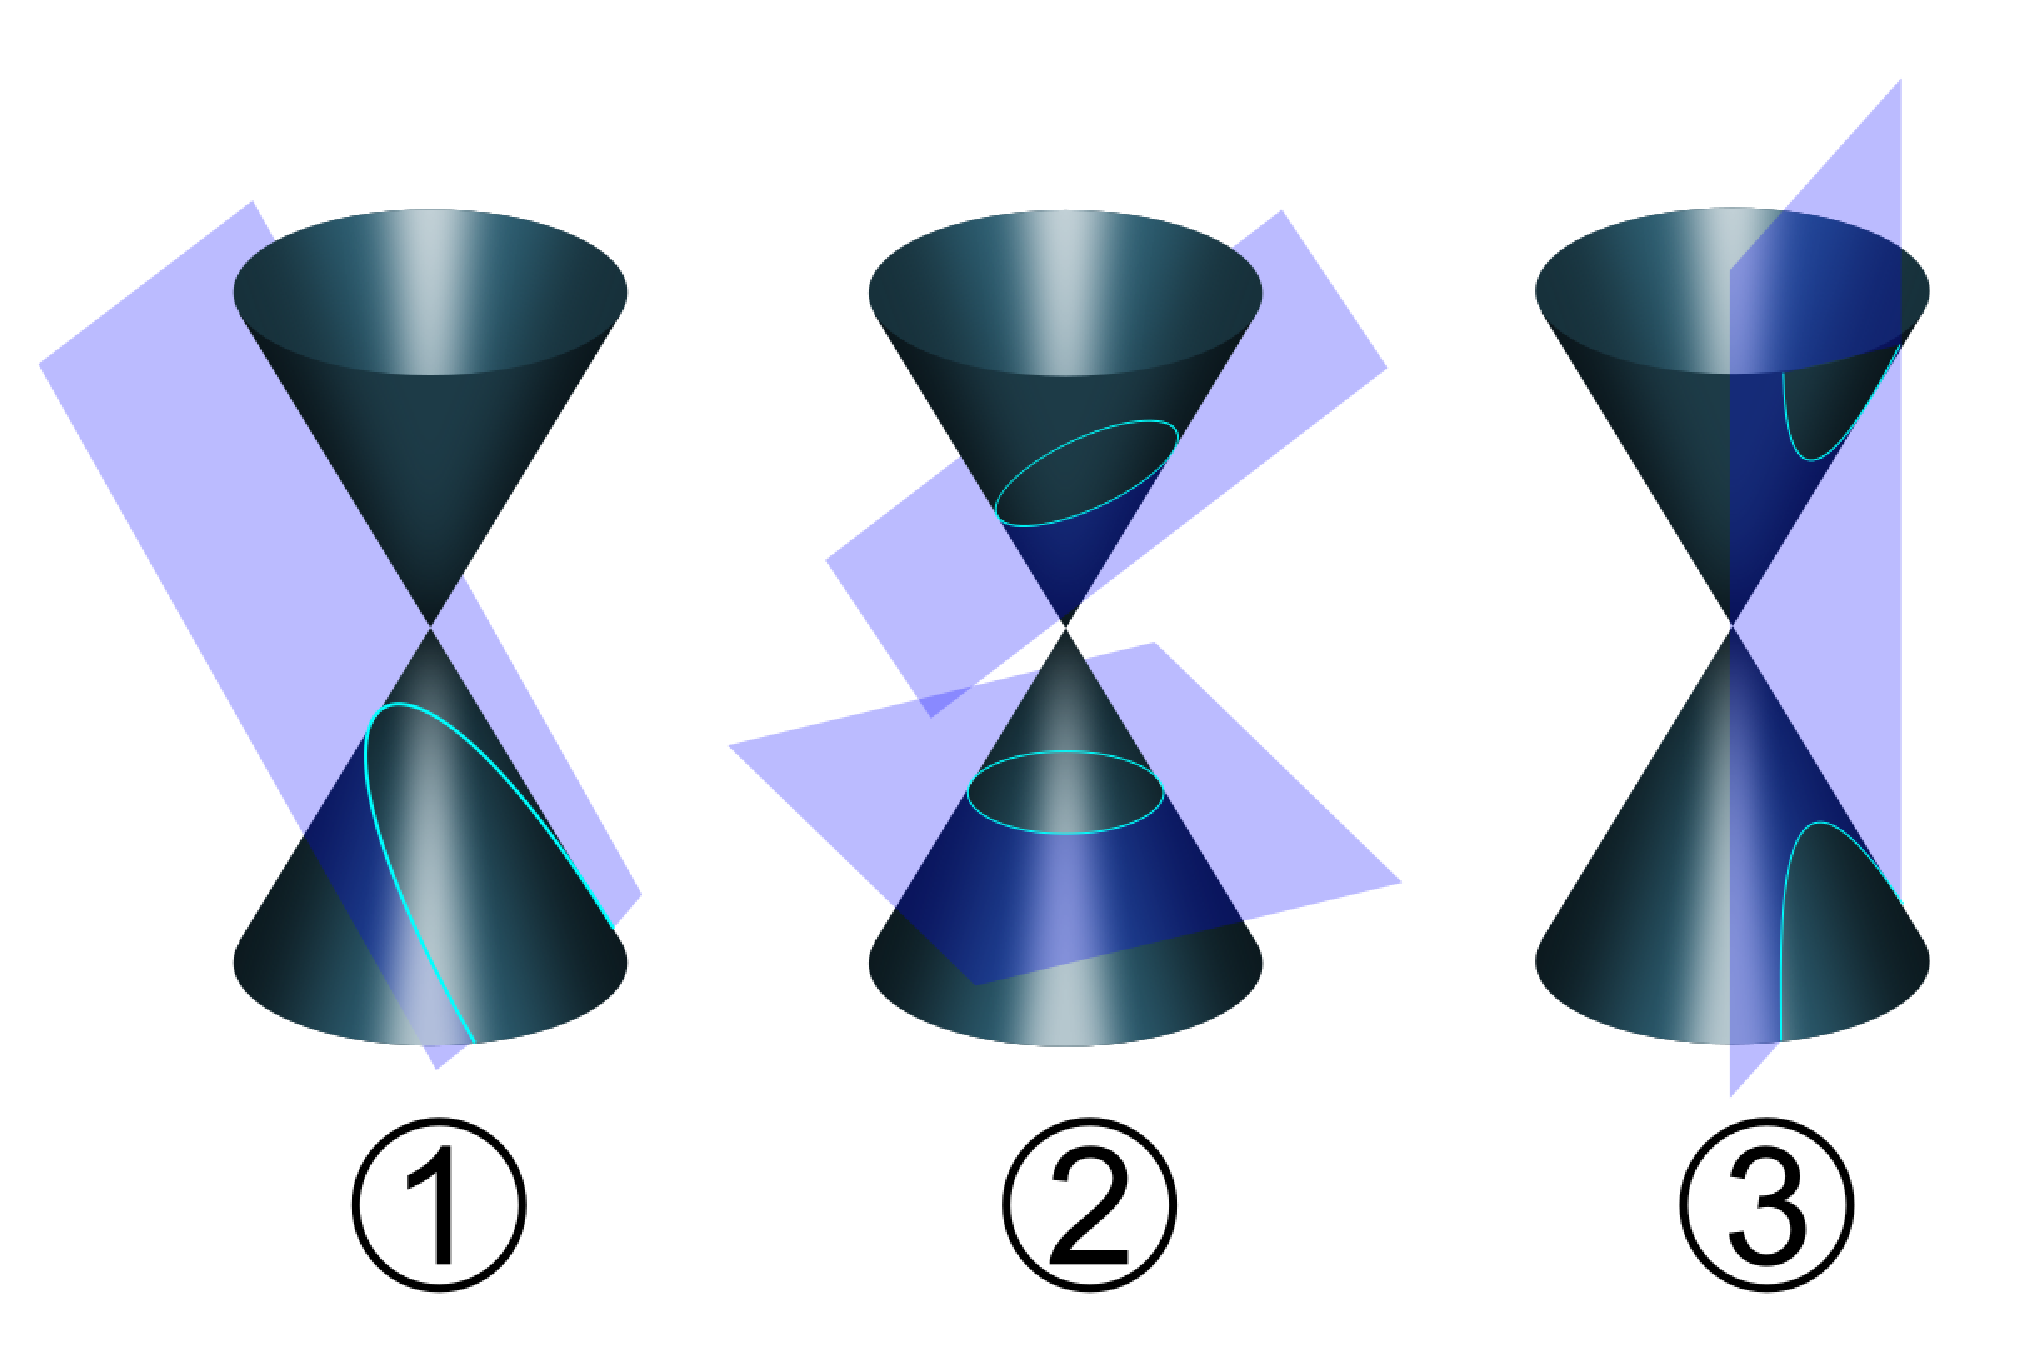
\includegraphics[width=1\linewidth]{conic_sections_with_plane.eps}}
    \end{wrapfigure}

    \[
        \begin{split}
            &B^{2} - 4 A C = 0 \\
            &B^{2} - 4 A C < 0 \\
            &B^{2} - 4 A C > 0
        \end{split}
    \]

\end{frame}

%SLIDE #
\begin{frame}{Каноническая форма уравнения}

    \transdissolve[duration=0.1]
    \justifying
    \large

    \begin{itemize}
        \item Каноническая форма уравнения гиперболического типа:
            \[
                \frac{\partial^{2} \phi}{\partial \xi^{2}} - \frac{\partial^{2} \phi}{\partial \eta^{2}} = h_{1} \left( \frac{\partial \phi}{\partial \xi}, \frac{\partial \phi}{\partial \eta}, \phi, \xi, \eta \right), \; \frac{\partial^{2} \phi}{\partial \xi \partial \eta} = h_{1} \left( \frac{\partial \phi}{\partial \xi}, \frac{\partial \phi}{\partial \eta}, \phi, \xi, \eta \right).
            \]

        \item Каноническая форма уравнения параболического типа:
            \[
                \frac{\partial^{2} \phi}{\partial \xi^{2}} = h_{2} \left( \frac{\partial \phi}{\partial \xi}, \frac{\partial \phi}{\partial \eta}, \phi, \xi, \eta \right).
            \]

        \item Каноническая форма уравнения эллиптического типа:
            \[
                \frac{\partial^{2} \phi}{\partial \xi^{2}} + \frac{\partial^{2} \phi}{\partial \eta^{2}} = h_{3} \left( \frac{\partial \phi}{\partial \xi}, \frac{\partial \phi}{\partial \eta}, \phi, \xi, \eta \right).
            \]
    \end{itemize}

\end{frame}

%SLIDE #
\begin{frame}{Системы уравнений}

    \transdissolve[duration=0.1]
    \justifying
    \large

    При изучении физических процессов обычно приходится решать \textbf{системы уравнений в частных производных}, так как редко удается описать сложный физический процесс одним уравнением в частных производных. Но даже в тех случаях, когда физический процесс описывается одним уравнением в частных производных высокого порядка, это уравнение можно заменить системой уравнений первого порядка.

\end{frame}

%SLIDE #
\begin{frame}{Пример №1}

    \transdissolve[duration=0.1]
    \justifying
    \large

%    Волновое уравнение $\frac{\partial^{2} u}{\partial t^{2}} - c^{2} \frac{\partial^{2} u}{\partial x^{2}} = 0$ может быть "факторизовано":
%
%    \[
%        \left[ \frac{\partial}{\partial t} - c \frac{\partial}{\partial x}\right] \left[ \frac{\partial}{\partial t} + c \frac{\partial}{\partial x} \right] u = 0.
%    \]
%
%    И может быть записанно в виде системы:
%
%    \[
%        \begin{cases}
%            &\frac{\partial u}{\partial t} + c \frac{\partial u}{\partial x} = v, \\
%            &\frac{\partial v}{\partial t} - c \frac{\partial v}{\partial x} = 0.
%        \end{cases}
%    \]

    Заменим волновое уравнение $\frac{\partial^{2} u}{\partial t^{2}} - a^{2} \frac{\partial^{2} u}{\partial x^{2}} = 0$ системой двух уравнений первого порядка. Обозначим

%    В волновом уравнении $\frac{\partial^{2} u}{\partial t^{2}} - c^{2} \frac{\partial^{2} u}{\partial x^{2}} = 0$ сделаем замену:

    \[
        \begin{split}
            &v = \frac{\partial u}{\partial t},\\
            &w = - a \frac{\partial u}{\partial x},
        \end{split}
    \]

%    тогда уравнение расщипится на систему двух уравнений:
    и рассмотрим систему уравнений

    \[
        \begin{cases}
            &\frac{\partial v}{\partial t} + a \frac{\partial w}{\partial x} = 0, \\
            &\frac{\partial w}{\partial t} + a \frac{\partial v}{\partial x} = 0. \\
        \end{cases}
    \]

    Подставляя вместо $w$ и $v$ их выражение через $u$, видим, что функция $u$ удовлетворяет волновому уравнению.

\end{frame}

%SLIDE #
\begin{frame}{Пример №2}

    \transdissolve[duration=0.1]
    \justifying
    \large

    Запишем уравнение Лапласа $\frac{\partial^{2} u}{\partial x^{2}} + \frac{\partial^{2} u}{\partial y^{2}} = 0$ в виде системы дифференциальных уравнений первого порядка:

    \[
        \begin{cases}
            &\frac{\partial u}{\partial x} = \frac{\partial v}{\partial y},\\
            &\frac{\partial u}{\partial y} = -\frac{\partial v}{\partial x}.
        \end{cases}
    \]

    Это известные уравнения Коши -- Римана, широко используемые в теории конформных отображений.

\end{frame}

%SLIDE #
\begin{frame}{Системы уравнений в частных производных первого порядка}

    \transdissolve[duration=0.1]
    \justifying
    \large

    Так как многие задачи математической физики сводятся к решению систем уравнений в частных производных первого порядка, то для корректной постановки задач необходимо уметь определять \textbf{тип системы уравнений в частных производных}. Рассмотрим систему линейных уравнений в частных производных первого порядка:

    \[
        \frac{\partial \mathbf{s}}{\partial t} + \mathbf{A} \frac{\partial \mathbf{s}}{\partial x} + \mathbf{B} \frac{\partial \mathbf{s}}{\partial y} + \mathbf{r} = 0.
    \]

\end{frame}

%SLIDE #
\begin{frame}{Условие гиперболичности системы уравнений в частных производных первого порядка}

    \transdissolve[duration=0.1]
    \justifying
    \large

    Системы уравнений в частных производных первого порядка называется \textbf{гиперболической} по $(x,t)$, если все \textbf{собственные значения} матрицы $\mathbf{А}$ \textbf{вещественны и различны}.\\

    То же самое можно сказать о поведении системы уравнений по $(y,t)$ в зависимости от собственных значений матрицы $\mathbf{B}$.

\end{frame}

%SLIDE #
\begin{frame}{Пример №3}

    \transdissolve[duration=0.1]
    \justifying
    \large

    В качестве примера рассмотрим систему уравнений из примера №1, записанную в виде:

    \[
        \frac{\partial \mathbf{s}}{\partial t} + \mathbf{A} \frac{\partial \mathbf{s}}{\partial x} = 0,
    \]

    где

    \[
        \mathbf{s}
        =
        \begin{bmatrix}
            u \\
            v
        \end{bmatrix}, \:
        \mathbf{A}
        =
        \begin{bmatrix}
            0 & a \\
            a & 0
        \end{bmatrix}.
    \]

\end{frame}

%SLIDE #
\begin{frame}{Пример №3}

    \transdissolve[duration=0.1]
    \justifying
    \large

    Собственные значения $\lambda$ матрицы $\mathbf{A}$ определяются из решения уравнения:

    \[
        \det \left| \mathbf{A} - \lambda \mathbf{I} \right| = 0.
    \]

    В нашем случае:

    \[
        \begin{Vmatrix}
            - \lambda & a \\
            a & - \lambda
        \end{Vmatrix}
        = 0
        \Rightarrow \lambda^{2} - a^{2} = 0
        \Rightarrow \lambda_{1,2} = \pm a.
    \]

    \begin{center}
        \textbf{Система гиперболическая!}
    \end{center}

\end{frame}

%SLIDE #
\begin{frame}{Условие эллиптичности системы уравнений в частных производных первого порядка}

    \transdissolve[duration=0.1]
    \justifying
    \large

    Системы уравнений в частных производных первого порядка называется \textbf{эллиптической} по $(x,t)$, если все \textbf{собственные значения} матрицы $\mathbf{А}$ \textbf{комплексные}.\\

    То же самое можно сказать о поведении системы уравнений по $(y,t)$ в зависимости от собственных значений матрицы $\mathbf{B}$.

\end{frame}

%SLIDE #
\begin{frame}{Пример №4}

    \transdissolve[duration=0.1]
    \justifying
    \large

    В качестве примера рассмотрим систему уравнений Коши -- Римана из примера №2, записанную в виде:

    \[
        \frac{\partial \mathbf{s}}{\partial x} + \mathbf{A} \frac{\partial \mathbf{s}}{\partial y} = 0,
    \]

    где

    \[
        \mathbf{s}
        =
        \begin{bmatrix}
            u \\
            v
        \end{bmatrix}, \:
        \mathbf{A}
        =
        \begin{bmatrix}
            0 & - 1 \\
            1 & 0
        \end{bmatrix}.
    \]

\end{frame}

%SLIDE #
\begin{frame}{Пример №4}

    \transdissolve[duration=0.1]
    \justifying
    \large

    Собственные значения $\lambda$ матрицы $\mathbf{A}$ равны:

    \[
        \begin{Vmatrix}
            - \lambda & - 1 \\
            1 & - \lambda
        \end{Vmatrix}
        = 0
        \Rightarrow \lambda^2 + 1 = 0
        \Rightarrow \lambda_{1,2} = \pm i.
    \]

    \textbf{Система эллиптическая!}

\end{frame}

%SLIDE #
\begin{frame}{Замечание №1}

    \transdissolve[duration=0.1]
    \justifying
    \large

    Система уравнений в частных производных первого порядка может оказаться \textbf{эллиптической} по $(y,t)$ и \textbf{гиперболической} по $(x,t)$ в зависимости от собственных значений матриц $\mathbf{B}$ и $\mathbf{A}$. Это связано с тем, что тип системы уравнений в частных производных первого порядка по $(x,t)$ и по $(y,t)$ определяется независимо.

\end{frame}

%SLIDE #
\begin{frame}{Замечание №2}

    \transdissolve[duration=0.1]
    \justifying
    \large

    Система уравнений, у которой часть собственных чисел вещественные, а часть комплексные, является смешанной и может обладать свойствами, характерными одновременно для гиперболических, параболических и эллиптических уравнений.\\

    Понять основные свойства решений систем уравнений смешанного типа обычно помогает знание описываемых ими физических процессов.

\end{frame}

\end{document}